\documentclass[11pt,xcolor=svgnames]{beamer}
\usepackage{dsfont,natbib,setspace,changepage,multirow,times}
\mode<presentation>

% fonts
\usepackage{pbsi}

% replaces beamer foot with simple page number
\setbeamertemplate{navigation symbols}{}
\setbeamercolor{frametitle}{fg=black}
\newcommand{\theme}{\color{Maroon}}

\setbeamertemplate{footline}{
   \raisebox{5pt}{\makebox[\paperwidth]{\hfill\makebox[20pt]{\color{gray}\scriptsize\insertframenumber}}}}

\usepackage{tikz}

\graphicspath{{/green/Dropbox/inputs/},
{/Users/mtaddy/Dropbox/inputs/},
{/home/taddy/project/bigdata/graphs/},
{/Users/mtaddy/project/bigdata/graphs/}}

\setbeamercolor{whitebox}{bg=gray!10}

% colors
\newcommand{\bk}{\color{black}}
\newcommand{\rd}{\color{red}}
\newcommand{\fg}{\color{ForestGreen}}
\newcommand{\bl}{\color{blue}}
\newcommand{\gr}{\color{black!60}}
\newcommand{\sg}{\color{DarkSlateGray}}
\newcommand{\br}{\color{SaddleBrown}}
\newcommand{\nv}{\color{Navy}}


% common math markups
\newcommand{\bs}[1]{\boldsymbol{#1}}
\newcommand{\mc}[1]{\mathcal{#1}}
\newcommand{\mr}[1]{\mathrm{#1}}
\newcommand{\bm}[1]{\mathbf{#1}}
\newcommand{\ds}[1]{\mathds{#1}}
\newcommand{\indep}{\perp\!\!\!\perp}

% spacing and style shorthand
\setstretch{1.1}

% shorthand
\newcommand{\sk}{\vspace{.5cm}}
\newcommand{\R}[1]{{\tt \nv #1}}
\newcommand{\til}{{\footnotesize$\bs{\stackrel{\sim}{}}$}}
\DeclareSymbolFont{extraup}{U}{zavm}{m}{n}
\DeclareMathSymbol{\vardiamond}{\mathalpha}{extraup}{87}

\begin{document}

\setcounter{page}{0}
{ \usebackgroundtemplate{
\includegraphics[height=\paperheight]{phoenix}}
\begin{frame}[plain]
\begin{center}


{\bf \Large [6] Big Data: Networks}

\vskip 1.5cm 
Matt Taddy, University of Chicago Booth School of Business

\vskip .2cm 
\texttt{faculty.chicagobooth.edu/matt.taddy/teaching} 


\end{center}
\end{frame} }


\begin{frame}
{[6] \theme Networks }

\sk
{Graphical models provide a language for networks: }
\\~~~0/1 
connections between people/sites/covariates.\\
~~~{\gr Think of graphs like a binary version of correlation.}
\vskip .25cm

{\bk Graph Structure:}
\begin{itemize}
\item Summarization: nodes and edges, direction.
\item Measuring connectivity and betweenness
\item Page Rank for relevance ordering.
\end{itemize}


\vskip .25cm
{\bk Association and networks}  
\begin{itemize}
\item Market Basket Analysis
\end{itemize}

\end{frame}

\begin{frame}

\sk
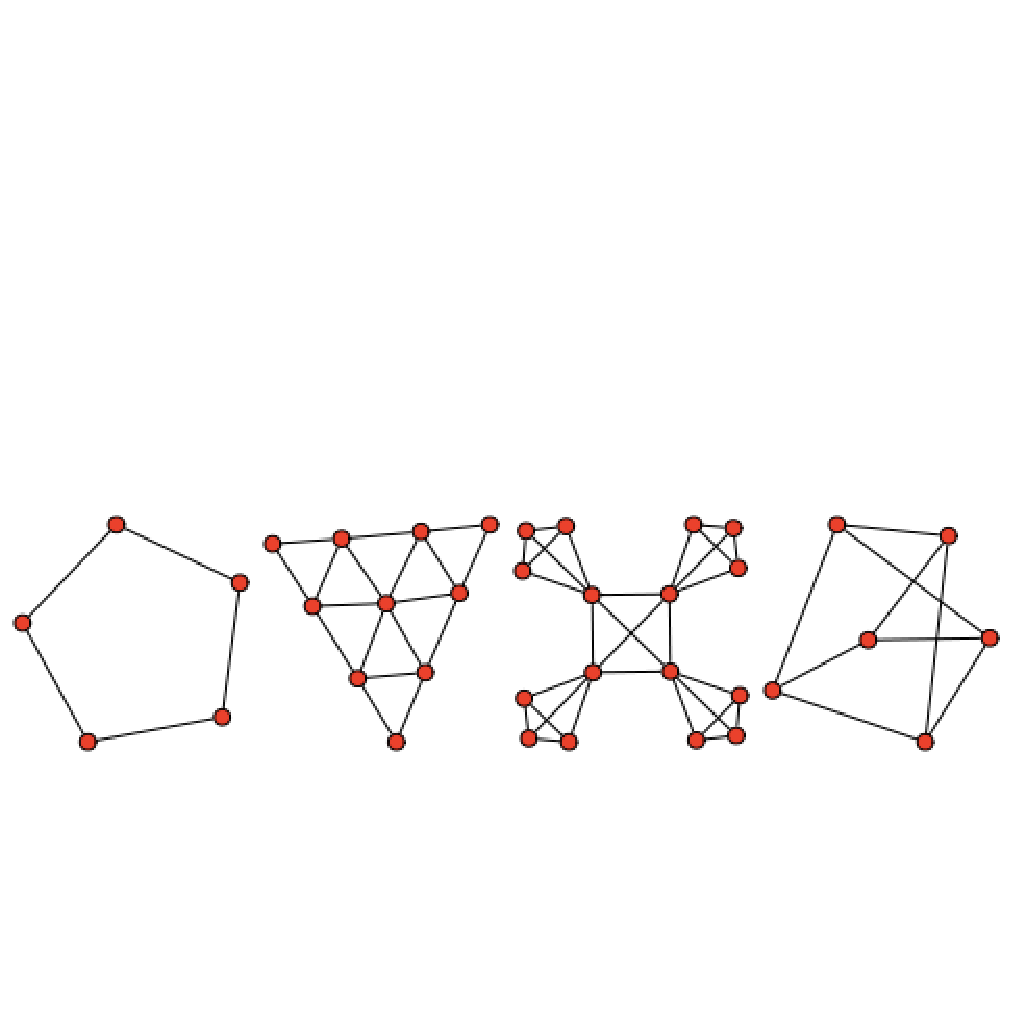
\includegraphics[width=4.25in]{../graphs/netgraphs1}

\sk
The network has {\nv nodes} (vertices){\gr, such as a website or
worker,}

\vskip .15cm

and {\nv edges} are the {\gr (directed or undirected)} links between nodes.

\sk
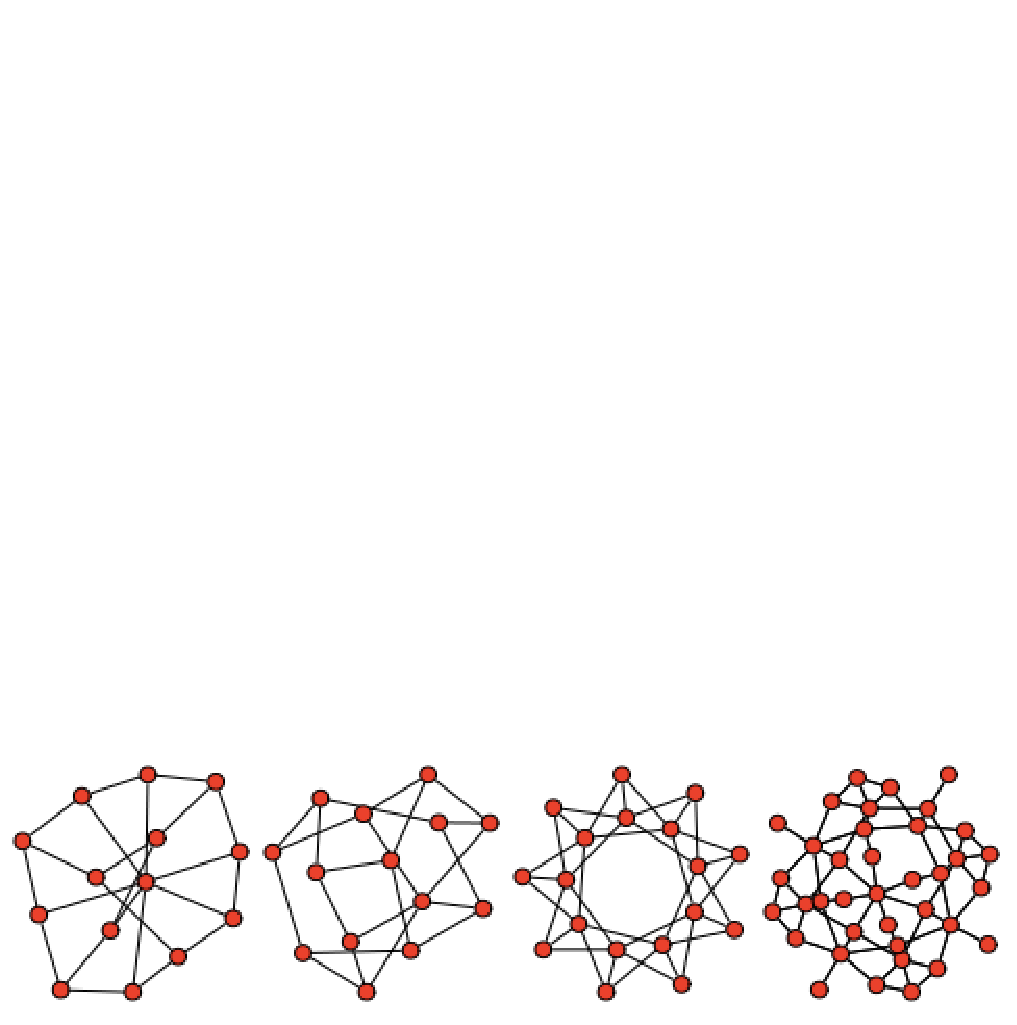
\includegraphics[width=4.25in]{../graphs/netgraphs2}
\vskip .25cm
\end{frame}

\begin{frame}
{Network data is connected}

\sk
A network consists of variables and connections between them.

{\nv 
A connection is discrete: it's either there or it's not.}\\


\sk
Data living on a network:
\begin{itemize}
\item Word usage in text and language {\gr (what words follow?)}
\item Organization charts and employment {\gr (who's boss?) }
\item Business credit, supply, and competition networks.
\item Genes: many SNPs pop if and only if another does.
\item {\nv Everything on the internet!}
\end{itemize}

\sk  \bk
Sometimes the network is given, \\other times we just glimpse {\it traffic} on the network.

\end{frame}

\begin{frame}
{Graph Models and Network Structure}


Start with a given network: you see all connections. \\

\vskip .1cm
We'll reduce dimension {\tt +} summarize important
  properties.

\vskip .1cm
In particular, we'll focus on measures of network {\nv connectivity}.

\vskip .5cm
Each node has connectivity statistics

\vskip .1cm
{\theme Degree}: How many other nodes are you connected to?

\vskip .1cm
{\theme Betweenness}: How many node-to-node paths go through you?

\sk You can also make a lot of cool illustrations for graphs.

\gr
These tend to be more pretty than informative, \\but that doesn't mean they aren't useful.

\end{frame}

\begin{frame}[fragile]

~\!{\bf \theme Network Graphs in R }

\vskip .25cm
\R{igraph} is a toolbox for visualizing and summarizing graphs.\\
It has front-ends for {\tt R} and {\tt Python}.
{\gr Others: Gephi, Pajek, etc.}

\vskip .25cm
Unlike most R packages, {\tt igraph} is well documented.  \\
Type {\tt help(igraph)} to get started.

\vskip .25cm
For most applications, you'll read graphs from an edgelist:


\begin{columns}

\column{1.5in}

\vspace{-.75cm}
\begin{verbatim}
              0  1
              0  2
              1  0
              2  1
\end{verbatim}

\column{.2in}
{\huge\gr $\Rightarrow$}

\column{2in}

\vskip .2cm
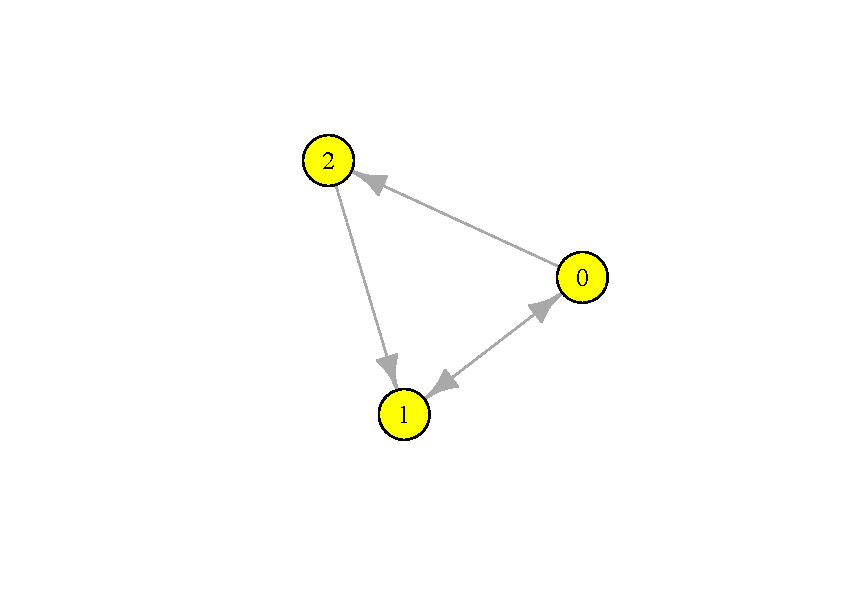
\includegraphics[width=1.1in]{../graphs/lilnet}
\end{columns}

{\nv
\begin{verbatim}
edgemat <- as.matrix(read.table("edgelist.txt"))
graph <- graph.edgelist(my_edgelist)
\end{verbatim}
}

\vskip -.5cm
\end{frame}

\begin{frame}

\begin{columns}

\column{3in}

\vskip -.1cm
\hskip -2cm 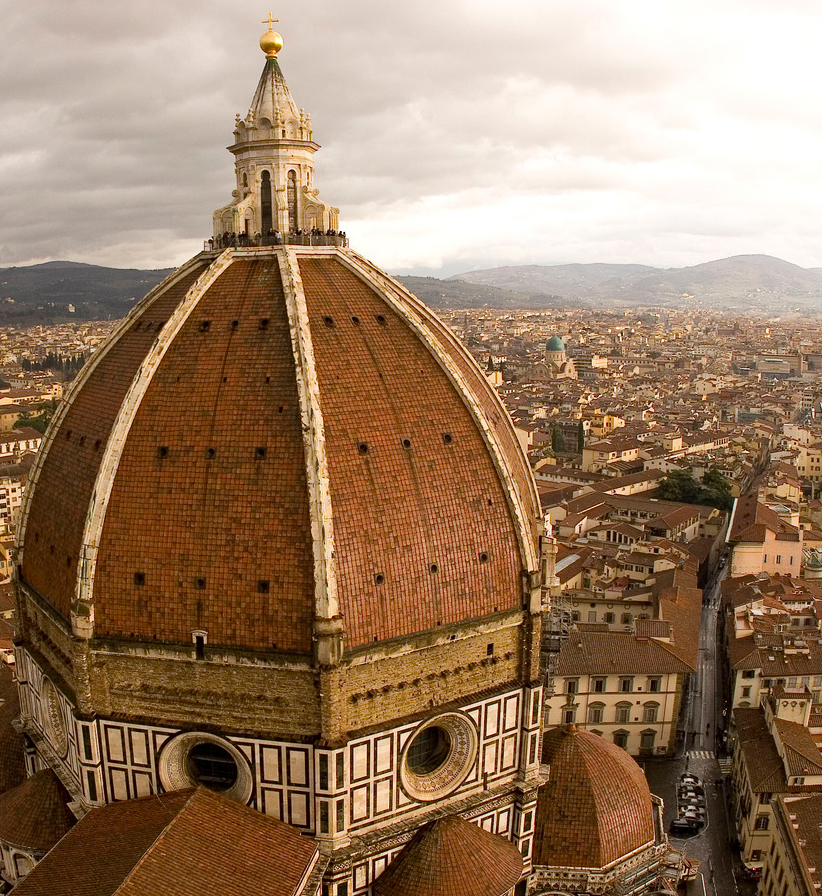
\includegraphics[width=3.5in]{../graphs/FRZpic}

\column{2in}

{\bf Marriage and Power}

\sk
Early Renaissance Florence was ruled by an oligarchy \\of
powerful families.

\sk 
By the 15th century, the Medicis emerged supreme,\\
\gr \& Medici Bank became\\ the largest in Europe.

\sk
Political ties were \\established via marriage.  \\ \theme How did Medici win?

\end{columns}

\end{frame}



\begin{frame}[fragile]


~\!{\bf Marriage in Florence: 1250-1450}

\begin{columns}

\column{2.25in}

\sk
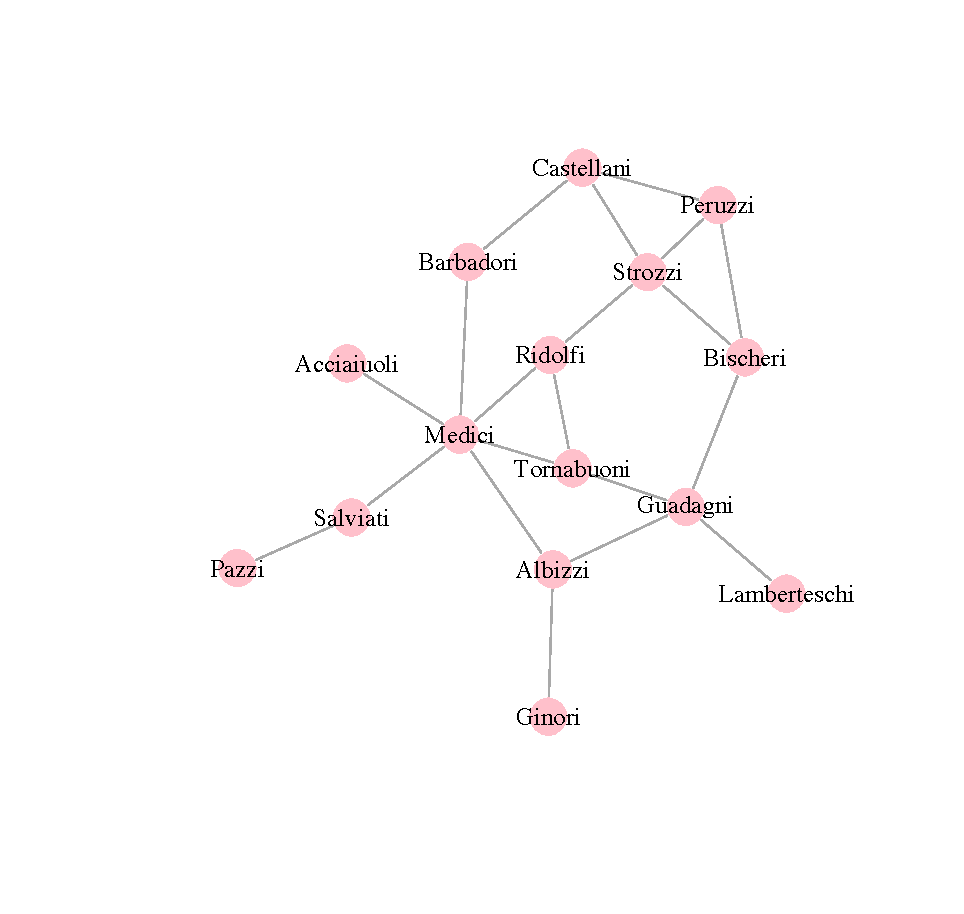
\includegraphics[width=2.5in]{../graphs/FRZnet}

\column{2in}

\sk
Network links can be used \\to measure ``social capital''.

\sk
{A node's {\theme degree} is\\
its number of edges.}\\

{\nv\small
\begin{verbatim}
> sort(degree(marriage))
Ginori ... Strozzi Medici 
     1           4      6
\end{verbatim}}


Medicis are connected!
\end{columns}

\sk
{\gr This is good enough for many analysis...}
\end{frame}



\begin{frame}

{\bf Deeper network structure with {\theme betweenness}}



\sk\bk
An alternative to degree, {\nv betweenness} measure the\\
proportion of {\nv shortest paths} containing a given node.


\sk
{\theme Shortest path:} fewest steps from $i$ to $j$ 
 {\gr (direction matters).}

\sk
\sg
Say $s_k(i,j)$ is the proportion of shortest \\paths from $i$ to
$j$ containing node $k$.
\[\nv
\text{betweenness}(k) = \sum_{i,j: i\neq j, k\notin \{i,j\}} s_k(i,j)
\]

\gr \hfill This measures how much influence a node \\\hfill has over connections between others.

\end{frame}

\begin{frame}[fragile]

\begin{columns}

\column{2in}

\sk
 { \bf Betweenness vs Degree}

\sk
Medicis have the highest degree,  but only by a factor of 3/2 over
the Strozzis.  


\sk {\theme
~~~But their betweenness\\ ~~~~is 5 times higher!}

\sk
Betweenness measures deep graph connectivity, rather than just
counting  neighbors.


\column{2.5in}

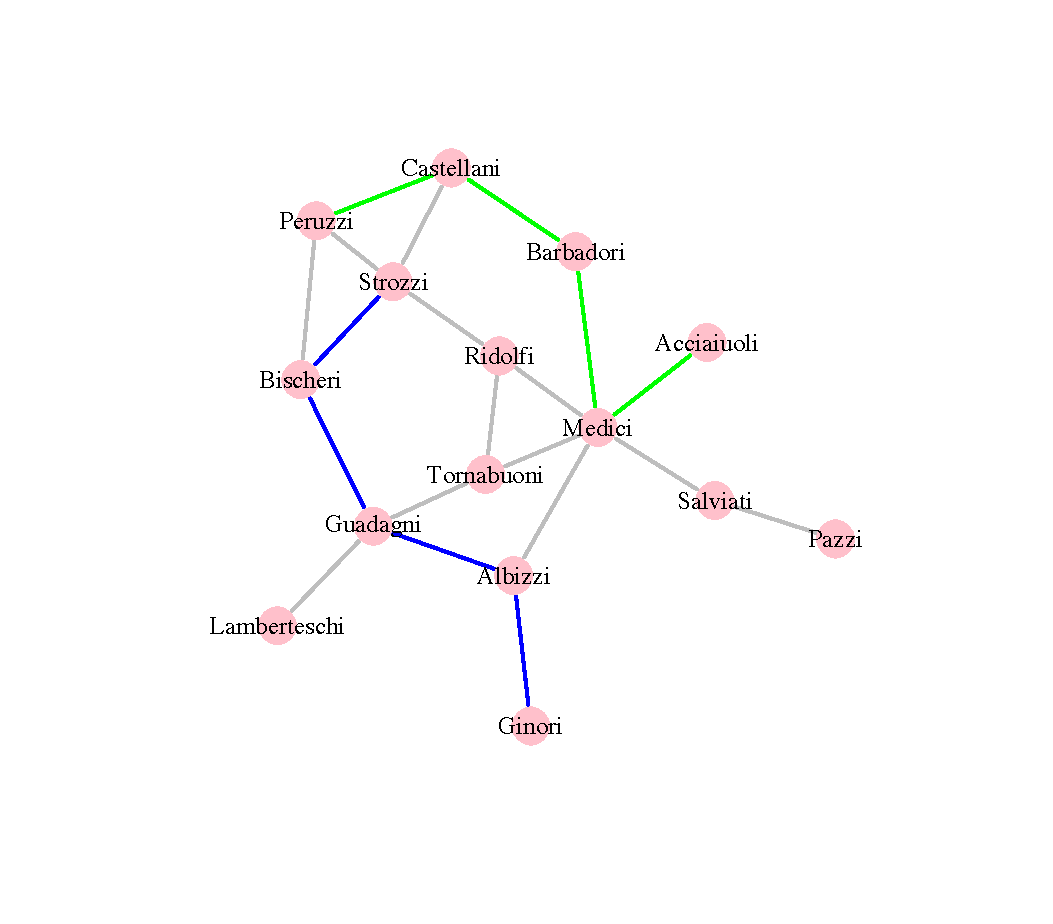
\includegraphics[width=2.5in]{../graphs/FRZshort}

\vskip -.25cm
{\nv\small
\begin{verbatim}
> sort(betweenness(marriage))
 Ginori  ...  Strozzi  Medici 
    0.0           9.3    47.5
\end{verbatim}}


\end{columns}


\vskip -.5cm
\end{frame}


\begin{frame}
{Structural Holes}

A structural hole is a low-level node in \\an organization chart with high betweenness.


\sk
Social Capital in brokerage opportunities.

{\sg The name seems pejorative, because it is. }

\vskip .1cm  Holes can act like
bottlenecks in companies, and lead to unexpected employees having
excess power and influence.

\vskip .1cm 
\nv But if you're the employee, it's a fast track to promotion!

\sk

\gr 
\hfill  Burt: {\it Structural Holes and Good Ideas}, AJS 2004.\\
\hfill {\tt igraph} has  {\tt constraint} for finding structural holes.

\end{frame}

\begin{frame}
{Collaborative Filtering}

A common question in data mining: \\ what do one person's choices say about anothers?

{\gr As amazon says: ``people who buy this book also bought...''}

\vskip .25cm
These types of tasks are referred to as `collaborative filtering': 

\hfill using shared choices to predict preferences.

\vskip .25cm  
It's a big field, with many tools
\begin{itemize}
\item logistic regression of each product on to all other choices.
\item principal componenets analysis: underlying taste factors.
\end{itemize}
Many of the tools from this class apply (projects?).

\vskip .25cm
But as an easy start, there are good fast algorithms \\for discovering low dimensional {\it association rules}.

\end{frame}

\begin{frame}
{Association Rules}

Consider two binary variables: $x_a$ {\tt+} $x_b$.\\ \hskip 1cm \bk
If $x_b =1$ more often when $x_a=1$, \\\hskip 1.5cm  then $x_a\Rightarrow x_b$ is an
association rule.


\sk
Ex: when you buy {\nv chips}, you need {\nv beer}
to wash them down.

\vskip .2cm
Suppose that beer is purchased 10\% of the time in general, but 50\% of the time when the consumer grabs chips.
\begin{itemize}
\item The {\it support} for `beer' is 10\%
\item The {\it confidence} of this rule is 50\%.
\item It's {\it lift} is 5: 50\% is 5 times higher than 10\%.
\end{itemize}

\vskip .2cm  Given this information, you could put some chips by the beer.

\end{frame}



\begin{frame}
{Market Basket Analysis}


{Using purchase coincidence to build association rules.}

\sk
Our example basket:{ \theme LHS {\gr (chips)}
$\Rightarrow$ RHS {\gr (beer)}} \\
Left Hand Side: `antecedent',  Right Hand Side: `consequent'.

\sk
{Every event has {\theme support}: the proportion of times it occurred.}
This leads to two measures of association rule strength: 

\vskip .25cm \bk
\begin{adjustwidth}{.2in}{}
{\theme confidence: } supp(LHS {\theme and} RHS)/supp(LHS)\\
{~~~~~~~~~~~~~~~~ The probability of {\nv RHS} given {\nv LHS}. }

\vskip .25cm
{\theme lift:} supp( LHS {\theme and} RHS )/[ supp(RHS) supp(LHS) ]\\
~~~~~~Increase in probability of {\nv RHS} given {\nv LHS} occurs.\\
\end{adjustwidth}
\end{frame}


\begin{frame}
{Support, Association, and Lift}


Generally, association rules with high {\nv lift} are most useful\\ because they
tell you something you don't already know.
\bk

\sk
Low {\theme support} does not preclude high {\theme confidence} or
high {\theme lift}.

\vskip .2cm\bk
{\nv Chips $\Rightarrow$ Beer} ~~is high support, but low lift if\\ 
~~~~~~~~~~~~~~~~~~~~~ everybody always buys beer.

\vskip .2cm
{\nv Caviar $\Rightarrow$ Vodka} ~~is low support, but high lift if people\\
~~~~~~~~~~~~~~~~~~~~~~~~
only buy vodka for their caviar parties.

\sk
There's no deep theory around ARules.  We just scan the high-lift or high-confidence rules to find interesting rules.

\end{frame}


\begin{frame}
{Finding Association Rules with R}


To find confidence and lift, just
count the number of times {\nv RHS} and {\nv LHS} happen, and how
often they happen together.

\[\theme 
\text{supp(event)} = \frac{\text{number of times event occurs}}{\text{number
of observations}}
\]

However, counting all possible combinations can take forever.  \\
{\nv Apriori:}   algorithm  for finding rules over
a support threshold.

\sk
 
The \R{apriori} function is available in the \R{arules} package.

\vskip .1cm
You need to get the data in a certain format, \\but after this it is straightforward to use.

\end{frame}

\begin{frame}

\begin{columns}

\column{3in}

 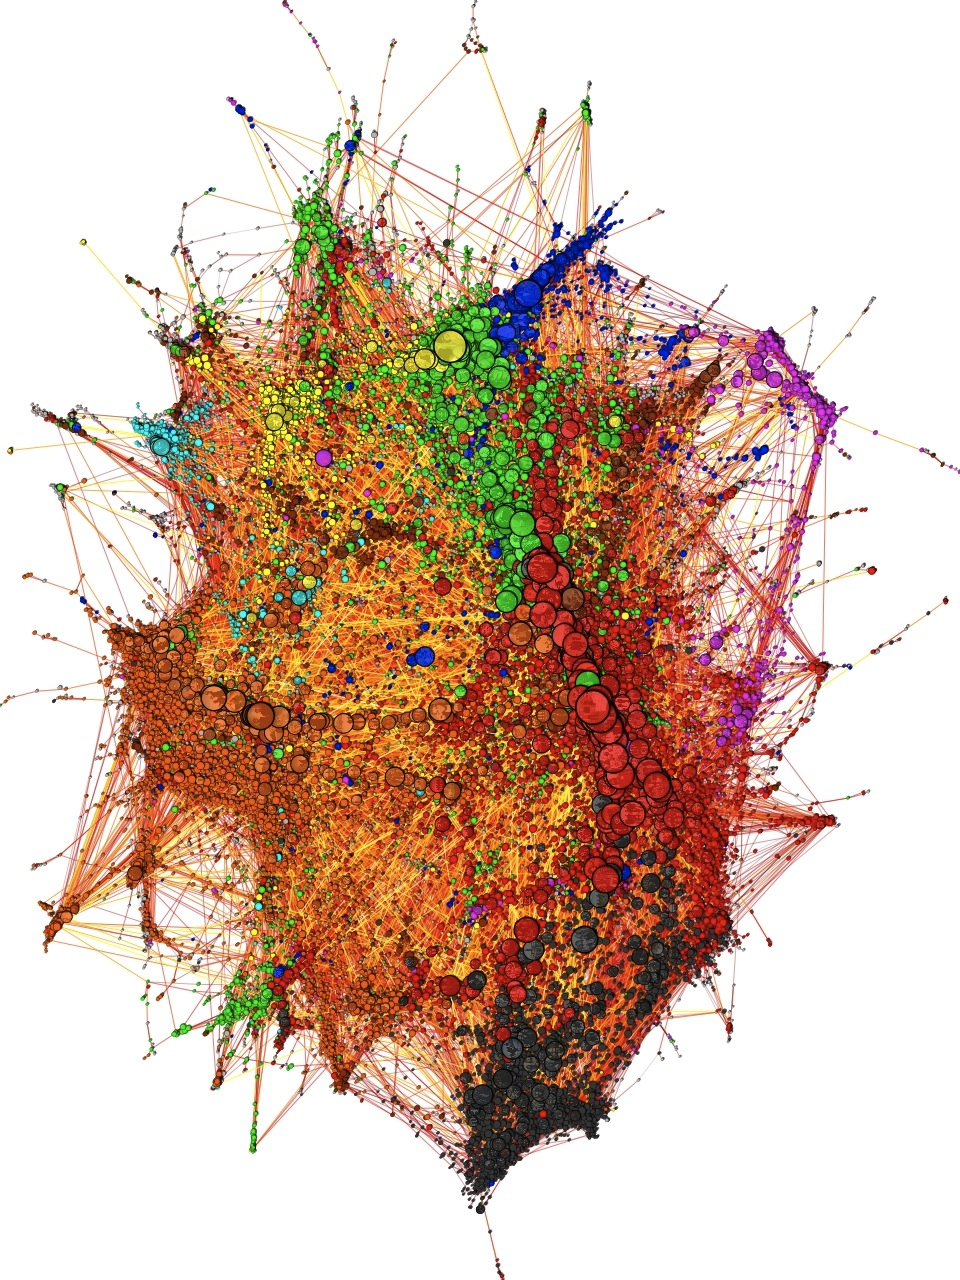
\includegraphics[width=2.8in]{lastfm_graph}

\column{2in}

\sk
{\theme\bf  Last.fm \bk Artist Plays}

\sk
Online radio keeps track

\vskip .1cm
 of everything you play, 

\vskip .1cm
for recommending music

\vskip .1cm
\& focused marketing.~~~~

\sk \sk\gr \footnotesize \hskip -.7cm This `network' shows artists
sized \\
\hskip -.7cm  by play 
count,
with lines (edges)\\

\vskip .1cm
\hskip -.7cm  for shared users. %\scriptsize \sg [ Tam\'as Nepusz ]

\vskip .5cm
\hskip -1.7cm {\bk metal}, {\rd rock}, {\fg pop}, {\color{Gold} jazz},
{\color{Orange} electronica}, {\bl hip-hop}\\
\hskip -1.7cm {\color{Magenta} reggae/ska}, {\color{cyan} classical}, {\color{Brown}
  folk/country/world}.  \\

\vskip .25cm
\hskip -3cm
\end{columns}

\end{frame}

\begin{frame}[fragile]
{Association rules for  Music Taste}

{\footnotesize \nv\vspace{-.5cm}
\begin{semiverbatim}
lhs                  rhs        support confidence lift
{t.i.}            => {kanye west}    0.0104  0.5672  8.8544
{pink floyd,                                               
 the doors}      => {led zeppelin}  0.0106  0.5387  6.8020
{beyonce}         => {rihanna}       0.0139  0.4686 10.8810
\theme{morrissey}       => {the smiths}    0.0112  0.4655  8.8961\nv
{megadeth}        => {iron maiden}   0.0132  0.4307  7.2677
{jimi hendrix}    => {the doors}     0.0120  0.3062  5.3170
{nelly furtado}   => {madonna}       0.0100  0.2750  5.0374
{bright eyes}     => {the shins}     0.0102  0.2698  5.4623
{elliott smith}   => {modest mouse}  0.0109  0.2679  5.1732
{britney spears}  => {lady gaga}     0.0120  0.2612  7.7292
{ramones}         => {the clash}     0.0104  0.2586  5.9052
{franz ferdinand} => {kaiser chiefs} 0.0132  0.2224  7.1153
\end{semiverbatim}}

{\gr Example:} \hfill Given a new user that listens to a lot of { Morrissey},\\
 \hfill  we're 46\% positive that they'll also like {the
   Smiths};

This is 9 times higher than if we didn't know about Morrissey.

\vskip -.25cm

\end{frame}

\begin{frame}[fragile]
{From association to networks}

{Graphs can be a useful way to summarize all sorts of data.}

We can define networks using any measure of connectivity.

\vskip .25cm
For example, an association network:

\vskip .1cm
~~~Say there's an edge between {\tt lhs} and {\tt rhs} if {\tt support} \\~~~and {\tt confidence} are greater than some thresholds.

\vskip .25cm{\gr
If we just look at any shared membership in a playlist,\\ we get our monster graph  from the beginning.}

\sk
For example, in the {\tt lastfm.R} code we use rules from
\begin{semiverbatim}\footnotesize\nv
apriori(playtrans, 
  parameter=list(support=.001, confidence=.1, maxlen=2))
\end{semiverbatim}
to define a network with 1k nodes and 36k edges.

\end{frame}

\begin{frame}

{\bf 0.1\% support and 10\% confidence lastfm network}

\sk
\begin{columns}

\column{2.75in}
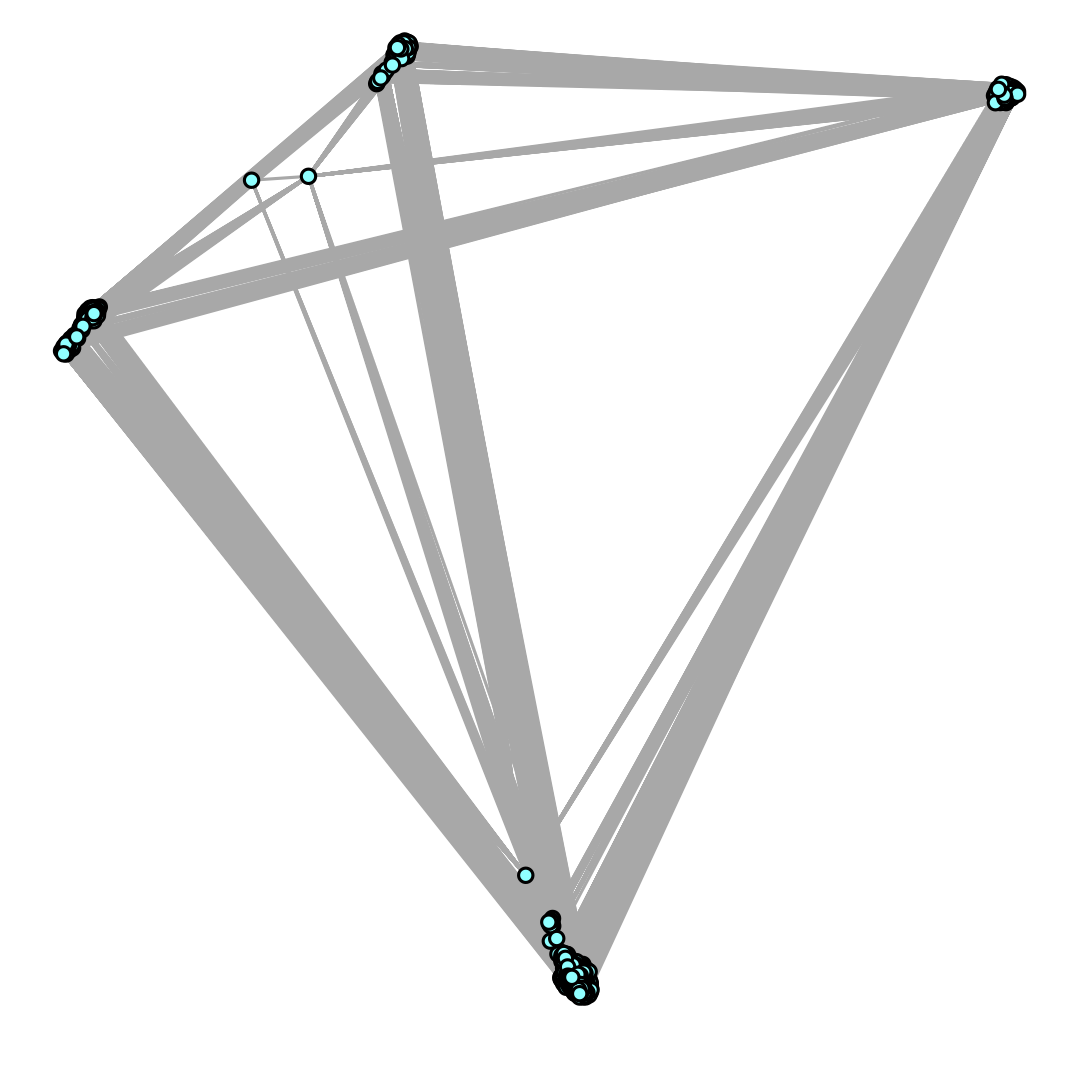
\includegraphics[width=3in]{musicnet}

\column{2in}

The network has four \\very distinct cliques.  

\vskip .25cm
These look something like {\it metal}, {\it hip-hop}, {\it alt}, {\it pop}.

\vskip .25cm
{\gr See code for plotting.  \\There's lots you can do.}


\end{columns}

\vskip -.5cm

\end{frame}

\begin{frame}[fragile]

{You can also focus in: a {\it neighborhood} of order $k$ for some node contains all vertices no more than $k$ steps away.}
\begin{columns}

\column{1.9in}
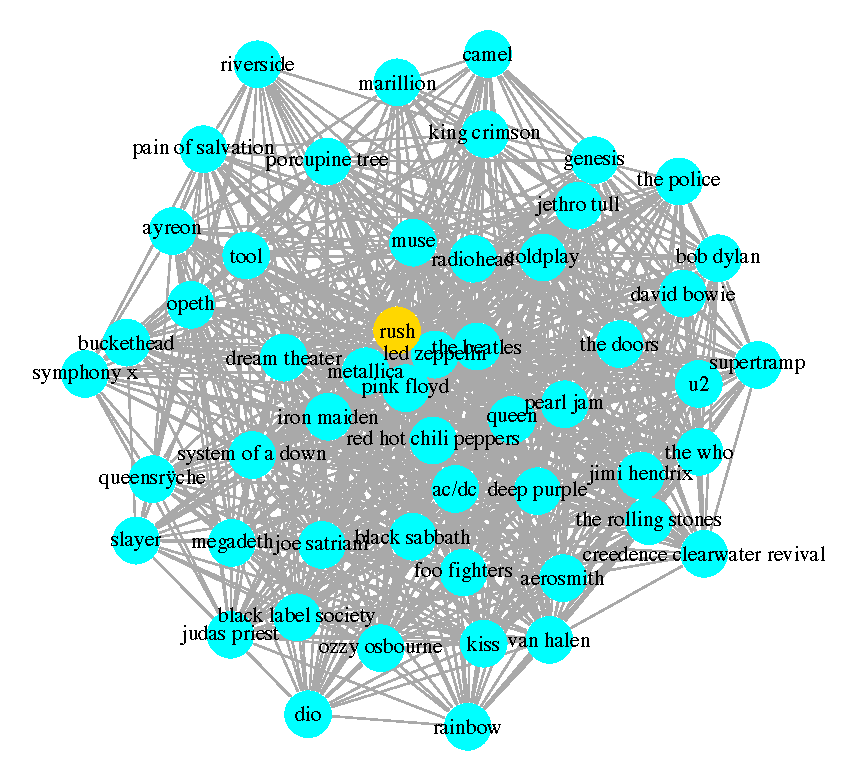
\includegraphics[width=3in]{rushnet}

\column{2.25in}

\vspace{-1in}
\begin{semiverbatim}\footnotesize\nv
nei <- graph.neighborhood(
      musicnet, order=1, 
      V(musicnet)["rush"])[[1]]
\end{semiverbatim}

\vspace{1.5in}
{\gr {\tt [[1]]} because it returns a list (you could look at multiple node neighborhoods at once)}
\vspace{-1in}

\end{columns}

\end{frame}

\begin{frame}[fragile]
{Connectivity in Music Choice}

{Popularity and connectivity are related but not the same}
\begin{semiverbatim}\footnotesize\nv
   > which.max(mbetween)  > which.max(playcount)\bk
       the beatles            radiohead 
\end{semiverbatim}

There is a strong connection, with some big outliers

\vskip .5cm
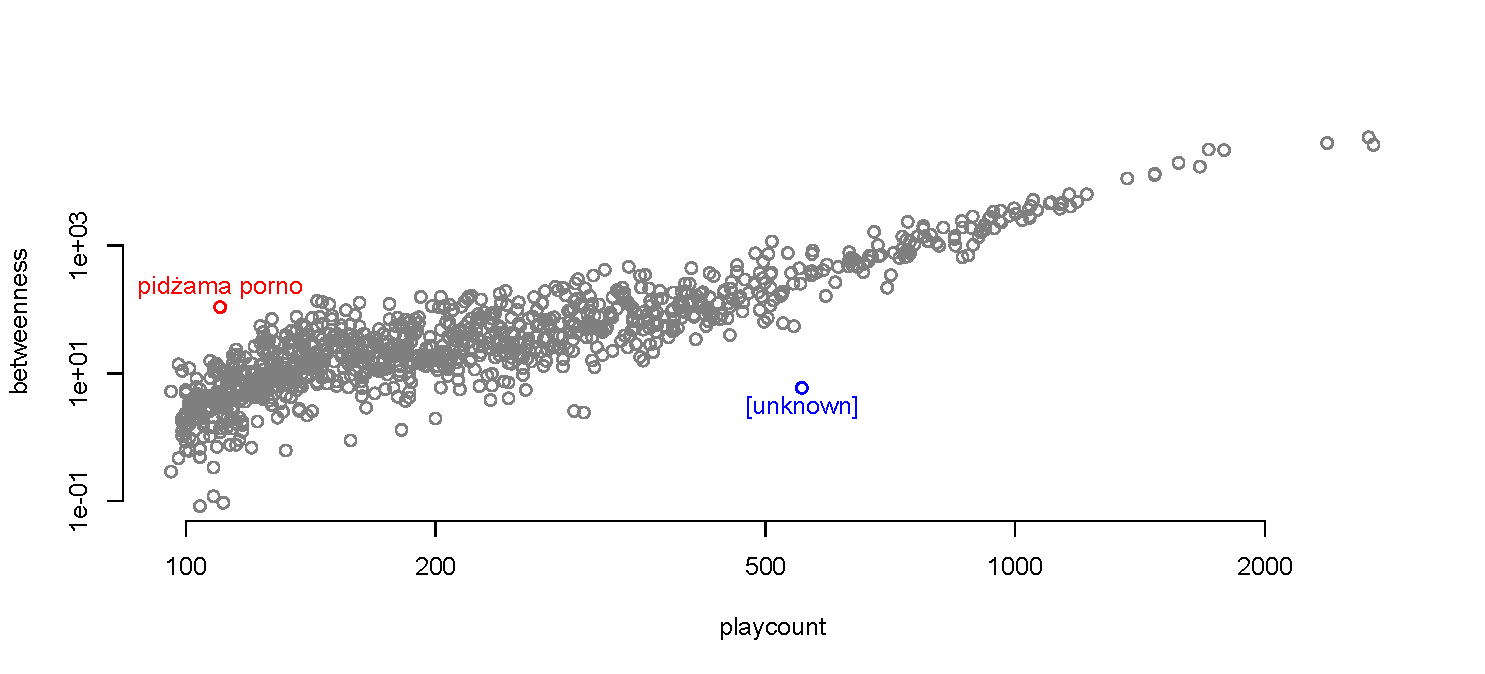
\includegraphics[width=\textwidth]{lastfmconnect}
\end{frame}

\begin{frame}[fragile]

~\!{\bf Search for ``{\theme california}'' }

\vskip -1.5cm
\hfill
\includegraphics[width=2.5in]{../graphs/bear}

\vskip .25cm
{\sg Search is one great example of network analysis;

Consider ranking sites for the query ``california''.}


\begin{adjustwidth}{.5in}{}
Expanding the response set:
\begin{itemize}\gr
\item Take 200 pages with heavy traffic and\\ high
term-frequency for ``california''.
\item Follow links to build a neighborhood.
\end{itemize}

We're left with about 10,000 sites, with links,  to rank.
\end{adjustwidth}

\vskip -.25cm

{\nv \footnotesize
\begin{verbatim}
caedges <- read.csv("CaliforniaEdges.csv")
casites <- scan("CaliforniaNodes.txt", "character")
edgemat <- cbind(casites[caedges$from], casites[caedges$to])
\end{verbatim}}

\vskip -2cm
\end{frame}


\begin{frame}[fragile]

{
The query provides a very large directed network}

{\gr Look at neighborhoods to get a workable plot.}

\vskip -.35cm
{\nv \footnotesize
\begin{verbatim}
latimes <- graph.neighborhood(calink, order=1, ...)
\end{verbatim}}

\vskip .5cm
{\bf {\theme LA Times} network} 

\vskip .75cm
Neighborhood order \\is  the number of \\ included steps away\\ from the node.

\vskip -1.9in
\hfill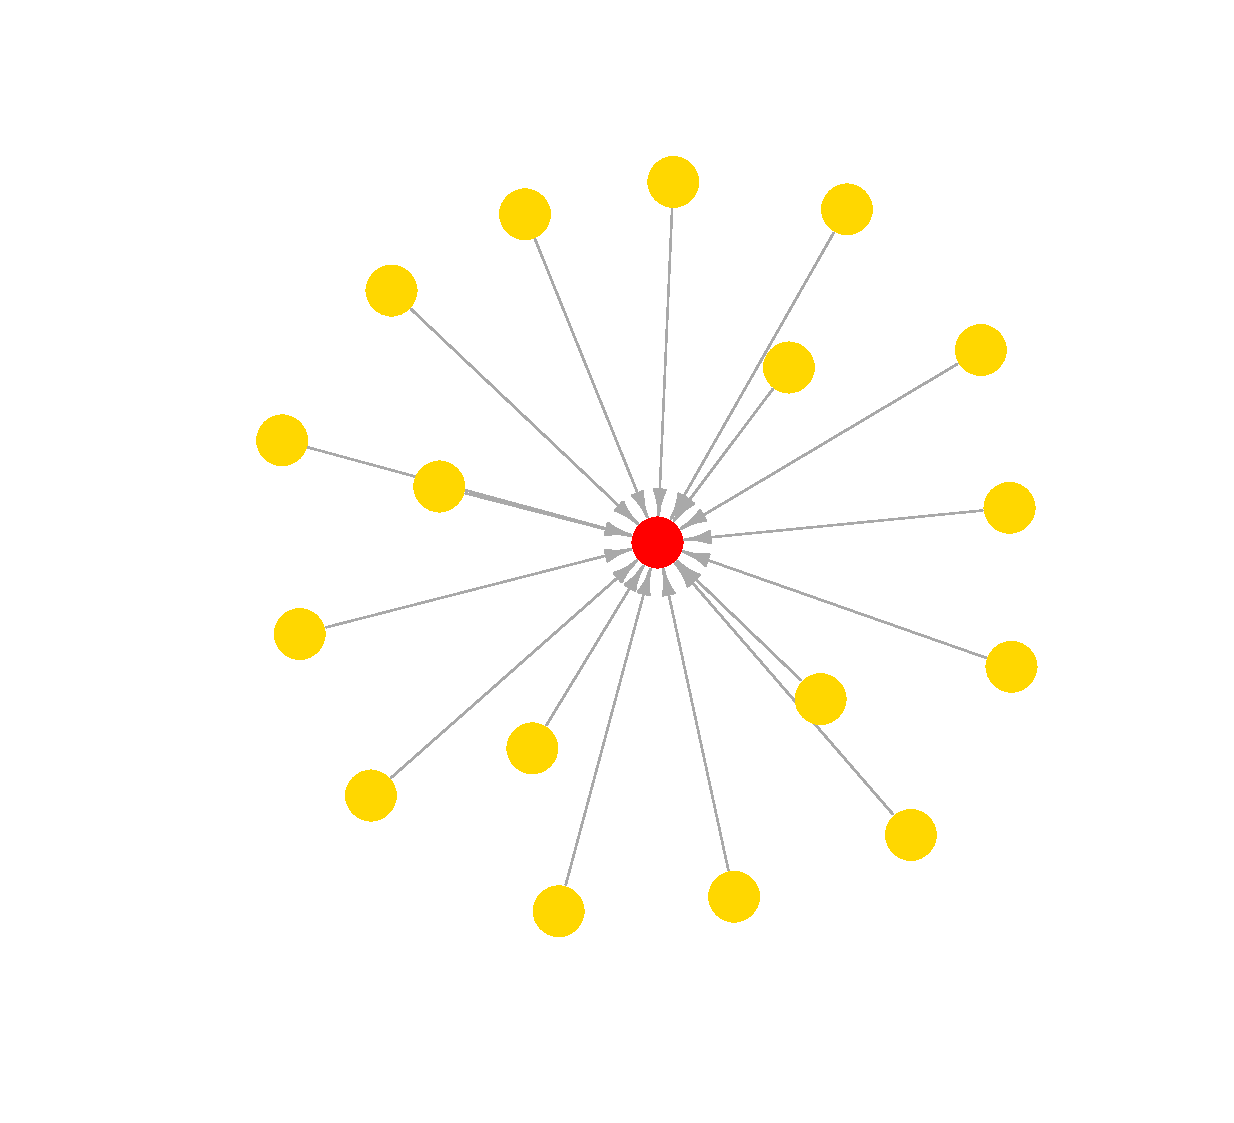
\includegraphics[width=3.2in]{../graphs/CAtimes}
  

\vskip -1cm\sg
At order=1, we just have sites pointing to {\tt latimes.com}.

\end{frame}

\begin{frame}

{\bf \bk LA Times Neighborhood \\ \theme  Expanded to order 2}

\vskip -.75in
\hfill~~~~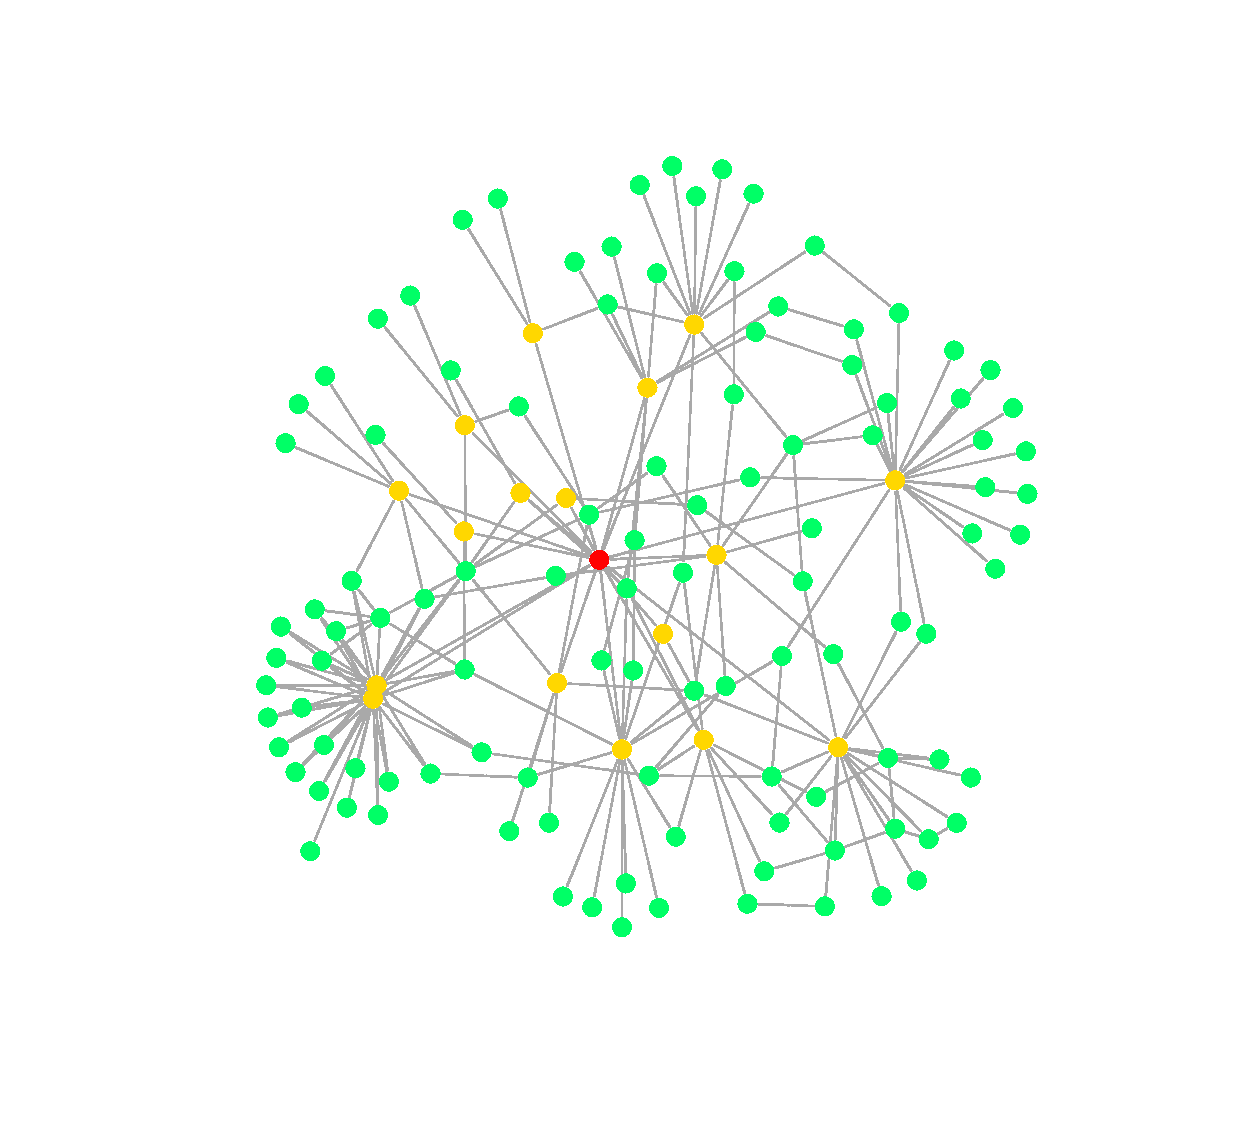
\includegraphics[width=4in]{../graphs/CAtimes2}\!\!\!\!\!\!\!\!\!

\vskip -1cm
{\sg
Just going one extra step creates a much bigger network.}\\
\gr Yellow points are the first-order connections from before.

\vskip -.5cm
\end{frame}


\begin{frame}

{\bf Larry and Sergei's \theme Page Rank}

\vskip .25cm


{\bl G\rd o\color{Gold}o\bl g\fg l\rd e}  has been pretty successful.  \\
Page Rank stat is a key ingredient.

\vskip .25cm
{\small {\nv Paper:} \gr The Anatomy of a Large-Scale \\Hypertextual Web Search
  Engine, 1998}

\sk \bk
Page Rank labels a site  more important if many sites link to it.\\
But the weight of each link is determined by its own rank.

\vskip .5cm
\theme ~~~~~~A recursive calculation:
$\displaystyle\large
r_i = \sum_{j=1}^n \frac{e_{ij}}{c_j}r_j$

\vskip .5cm
\bk \hfill $r_i$ is the page rank, $e_{ij}$ is a binary
  edge indicator, and \\\hfill $c_j = \sum_i e_{ij}$ is the number of nodes
  pointed at by node j.

\end{frame}

\begin{frame}[fragile]

~\!{\bf Page rank of ``{\theme california}'' search response}

\sk
We can run PageRank to organize our list of sites.

{\nv \scriptsize
\begin{verbatim}
          > search <- page.rank(calink)$vector
          > casites[order(search, decreasing=TRUE)]
           [1] "http://www.calgold.com/"                             
           [2] "http://www.sancarlos-homes.com/info.asp"             
           [3] "http://spectacle.berkeley.edu/"                      
           [4] "http://www.graddiv.ucr.edu/"                         
           [5] "http://www.chico-homes.com/info.asp"                 
           [6] "http://www.webb.pvt.k12.ca.us/~webb/WSCPrograms.html"
           [7] "http://www.berkeley.edu/"                            
           [8] "http://www.calfund.org/"                             
           [9] "http://www.ca-probate.com/"                          
          [10] "http://www.ppconline.com/"                           
\end{verbatim}}


I don't think this alone would have made google famous!  \\ Nodes need to be weighted by traffic and by \theme successful clicks.

\end{frame}


\begin{frame}
{Homework Due Next Week: Connectivity in Hollywood}

\small
We'll explore casts for `drama' movies from 1980-1999.  

See {\it actors} example code and data.\\
I've limited the data to actors in more than ten productions over this time period {\gr (and to movies with more than ten actors).}

\vskip .2cm
[1]  The actors network has an edge if the two actors were in the same movie.  Plot the entire actors network.

\vskip .1cm
[2]  Plot the neighborhoods for ``Bacon, Kevin'' at orders 1-3. \\ How does the size of the network change with order?

\vskip .1cm
[3]  
Who were the most common actors?  Who were most connected?
Pick a pair of actors and describe the shortest path between them.

\vskip .1cm
[4]  Find pairwise actor-cast association rules with at least 0.01\% support and 10\% confidence.  Describe what you find.

\vskip .1cm
{\gr [+] What would be a regression based alternative to ARules?  \\Execute it for a single RHS actor.}

\end{frame}




\end{document}
